\documentclass[a4paper,14.50pt]{book} \usepackage{color} \usepackage[usenames,dvipsnames,svgnames,table,x11names]{xcolor}
\usepackage{listings}
\usepackage[T1]{fontenc}
\usepackage{imakeidx}
\usepackage{graphicx}
\makeindex[columns=3, title=Alphabetical Index, intoc]
\usepackage{graphicx,wrapfig,lipsum}

\usepackage[hmargin=1cm, vmargin=3cm]{geometry}
\usepackage[font=tiny, labelfont=sc]{caption}
\usepackage{hyperref}

%get any font size by specifying a pt number
\usepackage{anyfontsize}

\usepackage[acronym]{glossaries}

\makeglossaries

\hypersetup{
    colorlinks=true,
    linkcolor=DeepSkyBlue4,
    urlcolor=blue,
    citecolor=blue,
    filecolor=blue
}

\renewcommand*{\glstextformat}[1]{\textcolor{black}{#1}}


\usepackage{tocloft}

\renewcommand{\cftpartfont}{\Large\bfseries\hypersetup{linkcolor=DeepSkyBlue4}}
\renewcommand{\cftsecfont}{\hypersetup{linkcolor=DarkSeaGreen4}}
\renewcommand{\cftsubsecfont}{\normalfont\hypersetup{linkcolor=LightCyan4}}
\renewcommand{\cftsubsecafterpnum}{\hypersetup{linkcolor=green}}

\newcommand{\wrapfill}{\par\ifnum\value{WF@wrappedlines}>0
  \addtocounter{WF@wrappedlines}{-1}%
  \null\vspace{\arabic{WF@wrappedlines}\baselineskip}%
  \WFclear
\fi}


\author{
  Daniele, Della Cioppa\\
  \texttt{daniele.dellacioppa@gmail.com}
}
\title{Rooting Android}

\renewcommand{\footnotesize}{\scriptsize}

\usepackage[utf8]{inputenc} % optional
\usepackage[T1]{fontenc}

% for underlining
%\usepackage{ulem}


%name of the chapter at every page 
\usepackage{fancyhdr}
\pagestyle{fancy}

\fancyhf{}
\fancyhead[RO,LE]{\textbf{\thepage}}
\fancyhead[LO]{\nouppercase{\textbf{\color{teal}\leftmark}}}
\fancyhead[RE]{\nouppercase{\textbf{\color{cyan}\rightmark}}}

%possibility to add chapters

\usepackage[english]{babel}

%background image to parts
\usepackage{eso-pic}

\usepackage{sectsty}    %package to define colors
\definecolor{Bluetto}{rgb}{0.2,0.4,1} %defining color
\definecolor{Bluettino}{rgb}{0.1,0.5,0.8} %defining color
\definecolor{Bluettetto}{rgb}{0.1,0.4,0.4} %defining color

\definecolor{LightBluetto}{rgb}{0.2,0.2,0.9}


\chapterfont{\color{Bluetto}}   %using the defined color for chapter fonts
\sectionfont{\color{Bluettetto}}  %defining section color
\subsectionfont{\color{Bluettino}} %defining subsection color
\subsubsectionfont{\color{teal}} %defining subsection color
\paragraphfont{\color{OliveGreen}} %defining paragraph color
\subparagraphfont{\color{LimeGreen}} %defining subparagraph color


%CODING BLOCKS


% -- Defining colors:
\usepackage[dvipsnames]{xcolor}
\definecolor{codegreen}{rgb}{0,0.6,0}
\definecolor{codegray}{rgb}{0.5,0.5,0.5}
\definecolor{codepurple}{rgb}{0.58,0,0.82}
\definecolor{backcolour}{rgb}{0.95,0.95,0.92}

\usepackage{caption}
\DeclareCaptionFont{teal!80}{\color{teal!80}}
%white che viene nel colorbox is a hack
\DeclareCaptionFormat{figure}{\colorbox{white}{\parbox{\textwidth}{#1#2#3}}}
%\captionsetup[lstlisting]{format=listing,labelfont=teal!80,textfont=teal!80}

%provo a definire le mie lstlisting captions
\DeclareCaptionFormat{listing}{\rule{\dimexpr\textwidth+17pt\relax}{0pt}\par\vskip1pt#1#2#3}
\captionsetup[lstlisting]{format=listing,singlelinecheck=false, margin=0pt, font={sf},labelsep=space,labelfont=bf,textfont=teal!80}
\captionsetup[figure]{format=default,singlelinecheck=true, margin=0pt, font={sf},labelsep=space,labelfont=bf,textfont=teal!80}




\lstdefinestyle{mystyle}{
    frame=lrb,
%     belowcaptionskip=4pt,
%     xleftmargin=8pt,
%     framexleftmargin=8pt,
%     framexrightmargin=5pt,
%     framextopmargin=5pt,
%     framexbottommargin=5pt,
%     framesep=0pt,
%     rulesep=0pt,
    backgroundcolor=\color{backcolour},   
    commentstyle=\color{codepurple},
    keywordstyle=\color{NavyBlue},
    numberstyle=\tiny\color{codegray},
    stringstyle=\color{codepurple},
    basicstyle=\ttfamily\footnotesize\bfseries,
    breakatwhitespace=false,         
    breaklines=true,                 
    captionpos=t,                    
    keepspaces=true,                 
    numbers=left,                    
    numbersep=5pt,                  
    showspaces=false,                
    showstringspaces=false,
    showtabs=false,                  
    tabsize=2
}
% -- Setting up the custom style:
\lstset{
  style=mystyle,
%  framexleftmargin=3.5mm,
  frame=shadowbox,
  rulesepcolor=\color{Sepia},
%  linewidth=0.6\linewidth,
%  xleftmargin=12pt,
%  aboveskip=12pt,
%  belowskip=12pt
}



% provo a definire il mio xml language
\lstdefinelanguage{XML}
{
  morestring=[b]",
  morestring=[s]{>}{<},
  morecomment=[s]{<?}{?>},
  stringstyle=\color{Indigo!70},
  identifierstyle=\color{BrickRed!70},
  keywordstyle=\color{cyan},
  morekeywords={xmlns,version,type}% list your attributes here
}

%quoting
\usepackage{csquotes}

%epigraph
\usepackage{epigraph} 

%fonts
%\usepackage[T1]{fontenc}
%\usepackage{accanthis}

\usepackage{fontspec}
%\renewcommand{\familydefault}{\rmdefault}
\setmainfont{FreeSerif}
%\setmainfont{MathJax_Fraktur} %per cose particuler


%possible wrapfig function
\newsavebox\curwrapfig
\makeatletter
\long\def\wrapfiguresafe#1#2#3{%
  \sbox\curwrapfig{#3}%
  \par\penalty-100%
  \begingroup % preserve \dimen@
    \dimen@\pagegoal \advance\dimen@-\pagetotal % space left
    \advance\dimen@-\baselineskip % allow an extra line
    \ifdim \ht\curwrapfig>\dimen@ % not enough space left
      \break%
    \fi%
  \endgroup%
  \begin{wrapfigure}{#1}{#2}%
    \usebox\curwrapfig%
  \end{wrapfigure}%
}
\makeatother

\def\simplewrap#1#2#3#4#5#6#7#8{%
\begin{wrapfigure}[#1]{#2}{#3}%
\centering%
\includegraphics[width=#4]{#5}%
\vspace{#6}%
\caption{#7}\label{#8}%
\end{wrapfigure}%
}

\definecolor{tecnico}{rgb}{0.4,0,0.4} %defining color

%#####funzione temporanea per riparare zone conflittuali
\def\conflictparagraph#1#2{%
\paragraph{\scalebox{#1}{#2}}\mbox{}\\
}
%#####fine funzione temporanea per riparare zone conflittuali

\def\techdata#1{%
\textbf{\color{tecnico}{\scalebox{1.3}{#1}}}
}

\definecolor{nometecnico}{rgb}{0,0.4,0.4} %defining color

\def\techname#1{%
\textbf{\color{nometecnico}{\scalebox{1.3}{#1}}}
}

\def\csquote#1{%
\begin{quote} 
\centering
\highlight{BrickRed!75}{#1}
\end{quote}
}

\def\freccetta#1{%
⇝ \textit{#1}%
}

\def\iniziocapitolo#1{%
\textbf{\scalebox{5}{\font\foo="Acorn Initials" \foo  #1}}%
}

\def\citazioneItaliana#1{%
\textbf{\scalebox{1.2}{\font\foo="Gracelya Script" \foo  #1}}%
}

\def\grazie#1{%
\textbf{\scalebox{0.9}{\font\foo="Gracelya Script" \foo  #1}}%
}

\def\workplace#1{%
\textbf{\font\foo="Glitten" \foo  #1}%
}

\def\suggerimento#1{%
\textbf{\font\foo="DejaVu Sans" \foo  #1}%
}


\definecolor{crystal}{rgb}{0.1,0.9,0.1} %defining color
\def\crystalname#1{%
{\color{crystal}{{#1}}}
}

\definecolor{docente}{rgb}{0.4,0.6,0.9} %defining color
\def\nomedocente#1{%
{\color{docente}{{#1}}}
}

\def\highlight#1#2{%
\textsc{\textbf{\color{#1}{#2}}}%
}


%\newacronym{hcf}{HCF}{Highest Common Factor}
%\newacronym{lcm}{LCM}{Lowest Common Multiple}
\newacronym{xml}{XML}{Extensible Markup Language}
\newacronym{rom}{\textsc{rom}}{\textbf{R}ead \textbf{O}nly \textbf{M}emory}
\newacronym{twrp}{\textsc{twrp}}{\textbf{T}EAM \textbf{W}in \textbf{R}ecovery \textbf{P}roject}
\newacronym{osi}{OSI}{Open Systems Interconnection}
\newacronym{ipv6}{IPv6}{Internet Protocol version 6}
\newacronym{ipv4}{IPv4}{Internet Protocol version 4}
\newacronym{RAID}{RAID}{Redundant Array of Indipendent disks}
\newacronym{DBMS}{DBMS}{\textbf{D}ata\textbf{B}ase \textbf{M}anagement \textbf{S}ystem}
\newacronym{ietf}{IETF}{Internet Engineering Task Force}
\newacronym{ipsec}{IPsec}{Internet Protocol Security}
\newacronym{sql}{SQL}{Structured Query Language}
\newacronym{ascii}{ASCII}{American Standard Code for Information Interchange}
\newacronym{utf8}{UTF-8}{\textbf{U}niversal Coded Character Set \textbf{T}ransformation \textbf{F}ormat \textbf{8}bit}
\newacronym{la}{LA}{Learning Assistant}
\newacronym{adt}{ADT}{Abstract Data Type}
\newacronym{ISO}{ISO}{\textbf{I}nternational \textbf{O}rganization for \textbf{S}tandardization}
\newacronym{gdpr}{GDPR}{\textbf{G}eneral \textbf{D}ata \textbf{P}rotection \textbf{R}egulation}
\newacronym{BCM}{BCM}{\textbf{B}usiness \textbf{C}ontinuity \textbf{M}anagement}

\newglossaryentry{SolutionLifeCycle}
{
    name=Solution Life Cycle,
    description={Set of stages software goes through from being an idea to implementation (discussed in \workplace{K1}\index{K1})}
}
\newglossaryentry{service-management-framework}
{
    name=Service Management Framework,
    description={Essential activities of good service management as processes or practices (discussed in \workplace{K2}\index{K2})},
    plural=Service Management Frameworks
}
\newglossaryentry{waterfall}
{
    name=waterfall,
    description={Simple methodology followed to develop in an old fashion. Discussed in \workplace{K2}\index{K2}}
}
\newglossaryentry{agile}
{
    name=agile,
    description={Incremental methodology to develop to adjust software to continuing changes in Requirements. Discussed in \workplace{K2}\index{K2}}
}
\newglossaryentry{bigdata}
{
    name=Big Data,
    description={Environments of storage for non relational structured and unstructured data (discussed in \workplace{K34}\index{K34})}
}
\newglossaryentry{table}
{
    name=table,
    description={Entity in which relational structured and unstructured databases store their data (discussed in \workplace{K33}\index{K33})},
    plural=tables
}
\newglossaryentry{dbms}
{
    name=\gls{DBMS},
    description={is covered in \workplace{K25}\index{K25}}
}
\newglossaryentry{android}
{
    name=Android,
    description={Popular Operating System running on most of the devices(covered in \workplace{K24}\index{K24})}
}
\newglossaryentry{DevOps}
{
    name=DevOps,
    description={approach discussed in \workplace{K3}\index{K3}}
}

\newglossaryentry{raid}
{
    name=RAID,
    description={concept present in \workplace{K41}\index{K41}}
}

\newglossaryentry{class}
{
    name=class,
    description={concept explained in Appendix \ref{appendix:class}. It's part of the \textsc{itsol} standards}
}

\newglossaryentry{object}
{
    name=object,
    description={(see Appendix \ref{appendix:class}) It is an instance of a class}
}

\newglossaryentry{array}
{
    name=array,
    description={DataType introduced in Appendix \ref{appendix:class}. It allows to store a raw of values of the same type}
}

\newglossaryentry{method}
{
    name=method,
    description={A type of function introduced in Appendix \ref{appendix:class}. It's a function that belongs to a specific class}
}

\newglossaryentry{router}
{
    name=router,
    description={concept present in \workplace{K11}\index{K11}},
    plural=routers
}

\newglossaryentry{switch}
{
    name=switch,
    description={concept present in \workplace{K11}\index{K11}},
    plural=switches
}

\newglossaryentry{firewall}
{
    name=firewall,
    description={a concept present in \workplace{K11}\index{K11}},
    plural=firewalls
}

\newglossaryentry{tcp}
{
    name=TCP,
    description={concept present in \workplace{K10}\index{K10}},
    plural=TCP
}

\newglossaryentry{iso}
{
    name=\gls{ISO},
    description={is an independent, non-governmental international organization with a membership of 167 \href{https://www.iso.org/members.html}{national standards bodies}}
}

\newglossaryentry{Java}
{
    name={Java},
    description={a programming language discussed in \workplace{K30}\index{K30}}
}

\newglossaryentry{C++}
{
    name={C++},
    description={a programming language discussed in \workplace{K30}\index{K30}}
}

\newglossaryentry{PHP}
{
    name={PHP},
    description={a programming language discussed in \workplace{K30}\index{K30}}
}

\newglossaryentry{Python}
{
    name={Python},
    description={a programming language discussed in \workplace{K30}\index{K30}}
}

\newglossaryentry{bcm}
{
    name=\gls{BCM},
    description={discussed in \workplace{K16}\index{K16}}
}







%leaving intentionally blank

\makeatletter
    \def\cleardoublepage{\clearpage%
        \if@twoside
            \ifodd\c@page\else
                \vspace*{\fill}
                \hfill
                \begin{center}
                \emph{This page intentionally left blank}
                \end{center}
                \vspace{\fill}
                \thispagestyle{empty}
                \newpage
                \if@twocolumn\hbox{}\newpage\fi
            \fi
        \fi
    }
\makeatother



% questo è per fare i teoremi

\usepackage[framemethod=TikZ]{mdframed}
%% the following is commaon for all examples in mdframed manual
\mdfsetup{skipabove=\topskip,skipbelow=\topskip}
%%% upto here
\newcounter{theo}[section]
\newenvironment{theo}[1][]{%
\stepcounter{theo}%
\ifstrempty{#1}%
 {\mdfsetup{%
   frametitle={%
    \tikz[baseline=(current bounding box.east),outer sep=0pt]
    \node[anchor=east,rectangle,fill=blue!20]
         {\strut Theorem~\thetheo};}}
 }%
{\mdfsetup{%
  frametitle={%
   \tikz[baseline=(current bounding box.east),outer sep=0pt]
   \node[anchor=east,rectangle,fill=blue!20]
        {\strut Theorem~\thetheo:~#1};}}%
 }%
\mdfsetup{innertopmargin=10pt,linecolor=blue!20,%
       linewidth=2pt,topline=true,
       frametitleaboveskip=\dimexpr-\ht\strutbox\relax,}
   \begin{mdframed}[]\relax%
}
{\end{mdframed}}




% altra dichiarazione di teoremi a se stante
\usepackage[many]{tcolorbox}
\newtcbtheorem[number within=section]{mytheo}{Theorem}%
  {colback=white,colframe=Bluetto!50,fonttitle=\bfseries,
   enhanced,
   coltitle=Bluetto!75!black,
   attach boxed title to top left=
     {xshift=2ex,yshift=-2mm,yshifttext=-1mm},
   boxed title style={colframe=Bluetto!50,
     colback=Bluetto!50}}{th}



% dichiarazione di definizione a se stante
\newtcbtheorem[number within=section]{mydef}{Definition}%
  {colback=white,colframe=Bluetto!50,fonttitle=\bfseries,
   enhanced,
   coltitle=LightBluetto!75!black,
   attach boxed title to top left=
     {xshift=2ex,yshift=-2mm,yshifttext=-1mm},
   boxed title style={colframe=LightBluetto!50,
     colback=LightBluetto!50}}{def}


% dichiarazione di suggerimento
\newtcbtheorem[number within=section]{myhint}{Hint}%
  {colback=white,colframe=BrickRed!50,fonttitle=\bfseries,
   enhanced,
   coltitle=black!75!blue,
   attach boxed title to top left=
     {xshift=2ex,yshift=-2mm,yshifttext=-1mm},
   boxed title style={colframe=BrickRed!50,
     colback=BrickRed!50}}{hint}


%###definizione hint()
\def\hint#1#2#3#4#5{%
\begin{wrapfigure}{#1}{#2}
\begin{tikzpicture}[node distance=5mm,
terminal/.style={
rectangle,
minimum size=6mm,
rounded corners=3mm,
very thick,
draw=BrickRed!40,
top color=BrickRed!30,
bottom color=orange}]
\node (norma) [terminal] at (0,0)
{
\begin{myhint}{#3}{#4}
\suggerimento{{\color{orange!75!black}#5}}
\end{myhint}
};

\node (azzurro)[xshift=-1.9ex,yshift=1.9ex] at (norma.south east)
{
\tikz \fill[orange, path fading=west] (2ex,2ex) circle (2ex);
};

\node (indaco) at (azzurro.center)
{
\tikz \fill[BrickRed!50] (1.8ex,1.8ex) circle (1.8ex);
};

\node (bianco) [xshift=-1ex,yshift=-0.3ex] at (norma.north east)
{
%\tikz \fill[white,opacity=.5] (1.8ex,1.8ex) circle (1.8ex);
\tikz \fill[white] (1.8ex,1.8ex) circle (1.8ex);
};

\node (idea) [yshift=0ex,xshift=0.3ex] at (bianco.center)
{
\includegraphics[width=1cm]{./chapters/english/idea.png}
};

\node (arancione) at (indaco.center)
{
\tikz \fill[blue] (0.8ex,0.8ex) circle (0.8ex);
};

\node (giallo) at (arancione.center)
{
\tikz \fill[white] (0.6ex,0.6ex) circle (0.6ex);
};

\end{tikzpicture}
\end{wrapfigure}
}
%###fine definizione hint()



%#######
%colori per la copertina

\definecolor{nometecnico}{rgb}{0,0.4,0.4} %defining color
\definecolor{lighttecnico}{rgb}{0.1,0.5,0.5} %defining color

\definecolor{marzullo}{HTML}{271a58}

\def\primotitolo#1{%
{\color{marzullo}\scalebox{2.6}{\textbf{\font\foo="Glitten" \foo  #1}}}%
}

\definecolor{davidita}{HTML}{543c7a}

\def\secondotitolo#1{%
{\color{davidita}\scalebox{2.4}{\textbf{\font\foo="Glitten" \foo  #1}}}%
}

\definecolor{rosalana}{HTML}{ec97bf}

\def\terzotitolo#1{%
{\color{rosalana}\scalebox{2.2}{\textbf{\font\foo="Glitten" \foo  #1}}}%
}
\definecolor{cristallo}{HTML}{4159a7}

\def\quartotitolo#1{%
{\color{cristallo}\scalebox{2.0}{\textbf{\font\foo="Glitten" \foo  #1}}}%
}
\definecolor{marechiaro}{HTML}{589a99}

\def\quintotitolo#1{%
{\color{marechiaro}\scalebox{1.8}{\textbf{\font\foo="Glitten" \foo  #1}}}%
}
%####### fine colori per la copertina


%#####capitolo idea
\usepackage{titlesec}
\newcommand{\chapnumfont}{
  \fontsize{144}{0}
  \selectfont
}

\colorlet{chapnumcol}{teal!55}

\titleformat{\chapter}[display]
{\bfseries}
{\begin{tikzpicture}
  \node[minimum width=\textwidth, text=teal!35, fill=teal!35, inner sep=1, outer sep=0, anchor=south ,xshift=-2cm] (rectinit) {\huge CHAPTER};
  \node[minimum width=.6\textwidth, text=white, inner sep=1, outer sep=0, anchor=south west, text width=.75\textwidth, align=right] at (rectinit.south west) (chapname) {\huge CHAPTER~~};
  \node[minimum width=.1\textwidth, inner sep=0, outer sep=0, anchor=south, text width=.1\textwidth, align=left, xshift=1cm] at (chapname.south east) {\chapnumfont\textcolor{chapnumcol}{\thechapter}};
\end{tikzpicture}}
{0pt}
{\Huge}
%#####fine capitolo idea








%######lista contenuti per ogni capitolo su due linee
\usepackage{minitoc}
%######fine lista contenuti capitolo su due linee


%annotation e ombre
\usetikzlibrary{shapes,shadows,calc}
\usetikzlibrary{mindmap}


%########tabella bella fatta in tikz ma non si integra nelle tikzpicture grandi
\usepackage{booktabs}

\usetikzlibrary{calc, backgrounds}

\newcommand\fancytab[4][]{%
\vspace*{\baselineskip}\noindent
\begin{minipage}{\linewidth}%
\captionsetup[table]{format=plain,skip=0pt,indention=0pt, font={color=white}}
\newlength{\mywidth}
\settowidth{\mywidth}{~#3+0}
#1
\begin{tikzpicture}
\node (around) {%
#4
};
\begin{scope}[on background layer]
\draw[pink, rounded corners, thick, fill=teal!10!pink!30,path fading=west] ($(around.north west)+(0,5mm)$) rectangle (around.south east);
\node[fill=teal, rounded corners, anchor=west, yshift=0mm, xshift=0.5mm, text width=\mywidth+0cm] at ($(around.north west)+(0,5mm)$) {\captionof{table}{#3}};
%\node[text=white, fill=pink] at (around.east) {$\clubsuit$};
\end{scope}
\end{tikzpicture}
\label{tab:#2}
\end{minipage}\par
\vspace*{\baselineskip}
\let\mywidth\relax % so we can reuse the same length
}
%########fine tabella bella fatta in tikz ma non si integra nelle tikzpicture grandi


%##########includiamo i pdf nel documento
\usepackage{pdfpages}
%########## fine di --- includiamo i pdf nel documento 


%#########funzione esempio a tre finestre
\def\tetraexample#1#2#3#4#5#6#7#8#9{
\begin{figure}[h]
\centering
\begin{tikzpicture}[node distance=5mm,
terminal/.style={
% The shape:
rectangle,
minimum size=0.1\linewidth,
% The rest
very thick,draw=white,
top color=white,bottom color=white,
font=\rmfamily},every annotation/.style={
minimum size=0.05\linewidth,
fill=BrickRed!45}]
\node (russell) [terminal] at (-8,0)
{
\lstinputlisting#1
};

\node (highlight) [rectangle,
    draw = black,
    thick,
    text = black,
%    path fading=north,
    rounded corners=1mm,
    fill = black,
    opacity=.2,
    minimum width = 56ex, 
    minimum height = #7,
    yshift=#8] at (russell.north)
{

};

\node (centro) [rectangle,
    draw = BrickRed,
    thick,
    text = black,
%    path fading=north,
    rounded corners=1mm,
    fill = BrickRed,
    opacity=.2,
    #9] at (highlight.center)
{

};

\node[inner sep=0pt,xshift=7cm] (whitehead) at (highlight.east)
    {#2};
\draw[->,thick] (highlight.east) -- (whitehead.west)
    #3

%\node (highlight) [annotation,scale=1,yshift=-9ex,xshift=8ex,path fading=north] at (russell.north)
%{
%
%};

\node (explaining) [annotation,scale=2,yshift=-1cm,xshift=-5ex,path fading=south,fill=BrickRed!30] at (whitehead.south)
{

{\fontsize{4.5pt}{2pt}\selectfont #5} 

};

\draw [->,thick,BrickRed] (centro.south) .. controls +(down:5mm) and +(left:5mm) .. (explaining.west)
            #4

\end{tikzpicture}
#6
\end{figure}
}


%#########fine esempio a 3 finestre


%##### immagini allineate con caption
\newcommand\img[4]{%
\hspace{1em}%
\vtop{%
\centering
\sbox0{\includegraphics[height=#3]{#1}}%
\hsize=\wd0
\linewidth=\hsize
\usebox{0}%

\captionof{figure}{#2}\label{#4}%
}%
\ignorespaces}
%#####FINE immagini allineate con caption

\geometry{paperwidth=512.87pt, paperheight=769.30pt}
\usepackage{fontawesome5} % pacchetto per includere le icone di Font Awesome 5

\sectionfont{\normalfont\Large\bfseries\color{marzullo}}

\makeatletter
\def\@seccntformat#1{\colorbox{marzullo}{\color{white}\csname the#1\endcsname}\hspace{5pt}}
\makeatother


\begin{document}
%---------------------------------------------COVER----------------------------------------------



\AddToShipoutPictureBG*{%
  \AtPageUpperLeft{%
    \raisebox{-\height}{%
      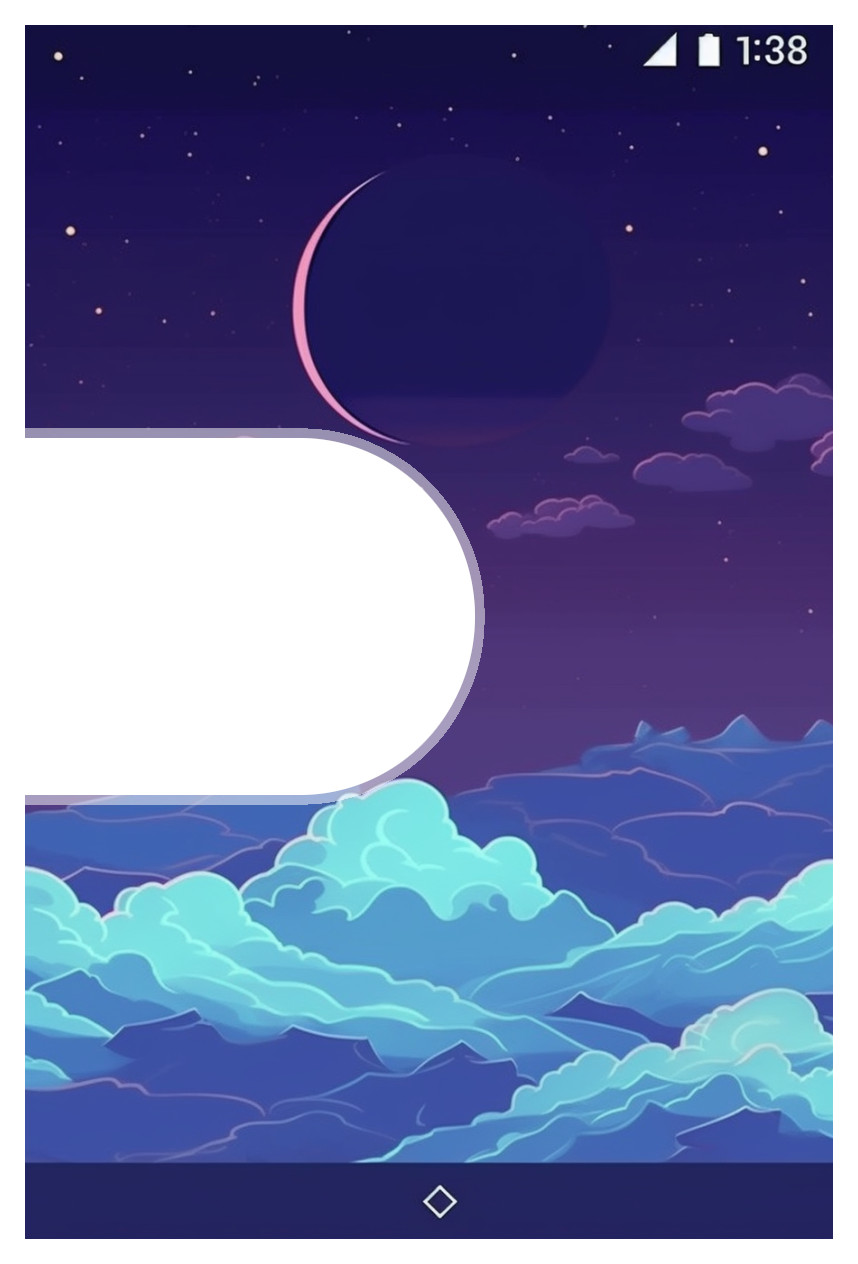
\includegraphics[width=\paperwidth]{./cover1.jpeg}%
    }%
  }
}

\pagenumbering{gobble}
\renewcommand{\headrulewidth}{0pt}



\begin{titlepage}
    \begin{center}
        \vspace*{6cm}
%        \hspace{12cm}            
        \Huge
        \noindent\makebox[\linewidth][l]{\primotitolo{Android Rooting}\hspace{10.2cm}}        
%        \vspace{0.5cm}
        \LARGE
%       \hspace{12.2cm}
%       \secondotitolo{Software Developer}
        \noindent\makebox[\linewidth][l]{\secondotitolo{Acer Tablet}\hspace{10.2cm}}
%        \vspace{1.5cm}
            
        \noindent\makebox[\linewidth][l]{\terzotitolo{ACTAB721}\hspace{10.2cm}}
%        \today
            
%        \vfill
        \vspace{1.5cm}        
        \noindent\makebox[\linewidth][l]{\quartotitolo{Daniele Della Cioppa}\hspace{10.2cm}}
        \noindent\makebox[\linewidth][l]{\quintotitolo{daniele.dellacioppa@gmail.com}\hspace{10.2cm}}
         
        \vspace{0.5cm}         
        \noindent\makebox[\linewidth][l]{\quintotitolo{\today}\hspace{10.2cm}} 
            
    \end{center}
\end{titlepage}
%########## fine copertina

%### quote
\vspace*{\fill} 
\begin{quote} 
\centering 
\scalebox{2}{\emph{For Giuseppe Mauro}} 
\end{quote}
\vspace*{\fill}
%### end quote

%###### about the author
\chapter*{\scalebox{5}{\color{black!50}\workplace{About the Author}}}

\begin{wrapfigure}{R}{0cm}
\begin{tikzpicture}[node distance=5mm,
terminal/.style={
% The shape:
rectangle,
minimum size=6mm,
rounded corners=3mm,
% The rest
very thick,
draw=black!50,
top color=white,
bottom color=black!20,
font=\ttfamily}]
\node (foto) [terminal] at (0,0)
{
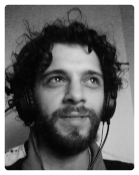
\includegraphics[width=3cm]{./chapters/author.png}
};

\node (rosso) [xshift=-1ex,yshift=1ex] at (foto.south east)
{
\tikz \fill[Indigo] (1ex,1ex) circle (1ex);
};

\node (arancione) at (rosso.center)
{
\tikz \fill[teal] (0.8ex,0.8ex) circle (0.8ex);
};

\node (giallo) at (arancione.center)
{
\tikz \fill[green] (0.6ex,0.6ex) circle (0.6ex);
};

\node (verde) at (giallo.center)
{
\tikz \fill[yellow] (0.4ex,0.4ex) circle (0.4ex);
};

\node (azzurro) at (verde.center)
{
\tikz \fill[orange] (0.2ex,0.2ex) circle (0.2ex);
};

\node (indaco) at (azzurro.center)
{
\tikz \fill[BrickRed] (0.1ex,0.1ex) circle (0.1ex);
};
%\simplewrap{16}{R}{5cm}{5cm}{}{-1pt}{D. Della Cioppa}{fig:author}
\end{tikzpicture}
\end{wrapfigure}

%\textbf{Daniele Della Cioppa} has been an IT Solutions student with \href{https://aclessex.com/about-us/}{ACL Essex}, developing IT skills across a variety of sectors to meet the needs of today’s workplace. He has designed and implemented TCP/IP-based apps in Android, PostgreSQL Databases following the SOLID principles. He is a language expert who runs the podcast \textbf{\emph{\href{https://open.spotify.com/show/05U0mbJEdy1PtqnXOTFHAR}{Speak Napolitano and Survive in Naples}}}. He has five languages under his belt and a lot of incredibly valuable tips to share on how to most effectively learn a language. 
%
%He became a fan of the Spaced Repetition System and of flashcards thanks to Kahei Lee and his incredible \href{https://www.poeticcantonese.com/}{Poetic Cantonese podcast}, where Kahei shares beautiful insights on the Cantonese language, letting the listener learn step by step. He also gained valuable insights from \href{https://coffeebreaklanguages.com/}{Mark Pentleton's podcast} on language learning techniques. Last but not least, \href{https://www.efficacemente.com/}{Andrea Giuliodori}'s book 'Studia meno studia meglio' has been a great resource for him in learning more efficient and effective study habits
%
%In his spare time he's working on independent projects to explore Android Operating systems capabilities, showcasing his best work on \href{https://danieledellacioppa.github.io/}{his webpage}

\textbf{Daniele Della Cioppa}, an IT Solutions student at \href{https://aclessex.com/about-us/}{ACL Essex}, has developed IT skills in various sectors to meet today's workplace demands. He has designed and implemented Android apps based on TCP/IP and PostgreSQL databases following the SOLID principles. Daniele is also a language expert who hosts a podcast called "\textbf{\emph{\href{https://open.spotify.com/show/05U0mbJEdy1PtqnXOTFHAR}{Speak Napolitano and Survive in Naples}}}," in which he shares valuable language-learning tips. With a proficiency in five languages, Daniele became a fan of the Spaced Repetition System and flashcards after listening to Kahei Lee's "\href{https://www.poeticcantonese.com/}{Poetic Cantonese}" podcast and Mark Pentleton's language-learning techniques podcast. Additionally, he has gained insights from Andrea Giuliodori's book "\href{https://www.efficacemente.com/}{Studia meno studia meglio}," which has helped him develop more efficient study habits. Daniele spends his spare time working on independent projects exploring the capabilities of Android Operating Systems, which he showcases on \href{https://danieledellacioppa.github.io/}{his webpage}.

%###### end about the author

%#### preface
\chapter*{\scalebox{5}{\color{black!50}\workplace{Preface}}}

{\fontsize{7pt}{2pt}\selectfont This book has been written in \LaTeX. The basal font used is FreeSerif.}

{\fontsize{7pt}{2pt}\selectfont \noindent All images contained in this book are generated using MidJourney and are the property of the author. Any unauthorized reproduction, distribution, or use of these images is strictly prohibited.}

\bigskip
\noindent \scalebox{2.5}{\color{black!50}\workplace{Why Create a Book on Android Rooting?}}
\bigskip

\noindent \tikz \fill[orange] (0.8ex,0.8ex) circle (0.8ex);
\noindent\workplace{\color{black!50}\scalebox{2}U}nderstanding the process of rooting an Android device can be a challenging task. Each device is a unique journey on its own, with no guarantee of reaching the desired destination. The decision to create a book on this topic stems from the need for organized and structured information, enabled by the power of LaTeX.

\noindent\tikz \fill[orange] (0.8ex,0.8ex) circle (0.8ex);
\noindent\workplace{\color{black!50}\scalebox{2}R}ooting an Android device is not a straightforward task, and it becomes even more challenging when you have only one device at your disposal. Each Android device has its unique specifications, hardware configurations, and software versions. Therefore, the rooting process can vary significantly from one device to another. What works for one device may not work for another, and the consequences of unsuccessful rooting attempts can be detrimental.

\noindent\tikz \fill[orange] (0.8ex,0.8ex) circle (0.8ex);
\noindent\workplace{\color{black!50}\scalebox{2}G}aining privileged access to the device's system files and functions through the process of rooting comes with inherent risks. Rooting may potentially void the device's warranty and, if not performed correctly, can result in system instability, data loss, or even bricking the device entirely. When you have only one device, the stakes are higher as you lack the convenience of a backup device to rely on in case of any issues or failures.


\noindent\tikz \fill[orange] (0.8ex,0.8ex) circle (0.8ex);
\noindent\workplace{\color{black!50}\scalebox{2}E}ach manufacturer and carrier imposes different restrictions and security measures on their devices, making the rooting process even more intricate. Some devices have locked bootloaders, which adds an extra layer of complexity to gaining root access. Additionally, system updates and security patches released by manufacturers can render previously working rooting methods ineffective, necessitating the exploration of new techniques and exploits.

\noindent\tikz \fill[orange] (0.8ex,0.8ex) circle (0.8ex);
\noindent\workplace{\color{black!50}\scalebox{2}N}avigating the world of Android rooting requires in-depth technical knowledge and a thorough understanding of the device's specific architecture and software. It involves working with complex commands, custom recovery tools, and potentially modifying critical system files. Without proper expertise and guidance, attempting to root a device can result in irreversible damage.

\noindent\tikz \fill[orange] (0.8ex,0.8ex) circle (0.8ex);
\noindent\workplace{\color{black!50}\scalebox{2}T}he decision to create a comprehensive book on Android rooting stems from the recognition that having organized and reliable information is crucial in tackling this challenging endeavor. By documenting the journey, sharing experiences, and providing step-by-step instructions, this book aims to serve as a valuable resource for those willing to explore the world of rooting, while also emphasizing the importance of caution, research, and understanding the specific risks and implications involved.





%####end preface


\dominitoc% Initialization mini lista contenuti per capitolo
\tableofcontents


%\clearpage
\cleardoublepage

\title{%
Android Rooting\\
\large  Acer Tablet\\
\small model n. ACTAB721}
\maketitle
\hypersetup{linkcolor=blue}

%\part{English Functional Skills}

\pagenumbering{arabic}
\renewcommand{\headrulewidth}{0.2pt}

\part{Preparation}
{\color{teal}\chapter{Initial Steps}\label{cap:dpa}}

\minitoc

\AddToShipoutPictureBG*{%
  \AtPageUpperLeft{%
    \raisebox{-\height}{%
      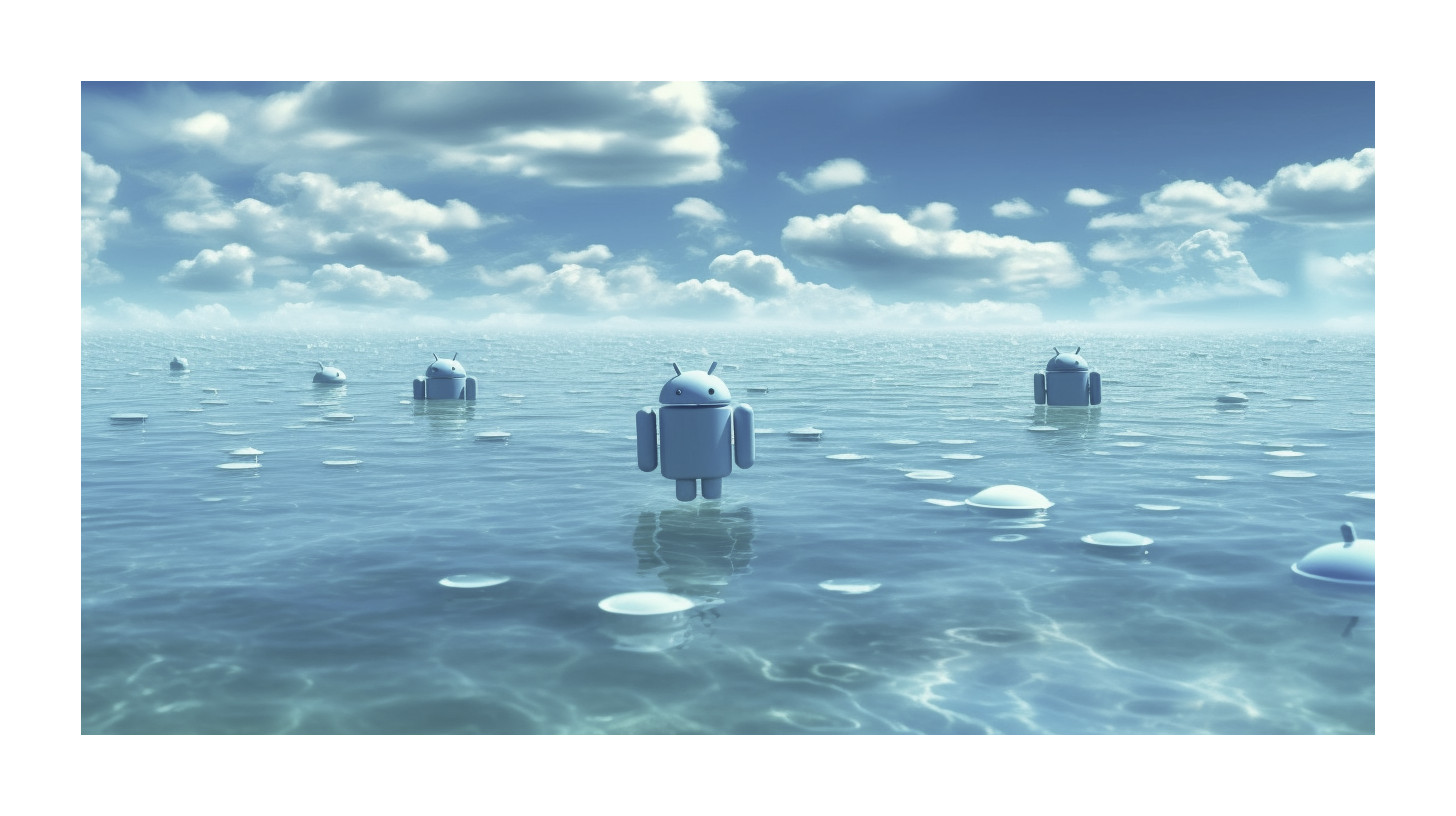
\includegraphics[width=\paperwidth]{./chapters/initialsteps/cover.jpeg}%
    }%
  }
}

\section{Let's Get Started}{\faCaretRight}
Welcome to the "Let's Get Started" section for exploring the rooting of the ACTAB721 device! Before we begin, it's important to understand that rooting carries risks and may void your device's warranty. Make sure you understand the risks involved and proceed with caution.

\subsection{Introduction to Rooting}

Rooting is the process of obtaining administrator privileges (root access) on your Android device. It grants you greater control over the operating system, allowing for deep customization and modification of your device. However, please be aware that rooting comes with risks, such as data loss, device malfunctioning, and compromised security. Exercise caution and be aware of the potential negative impacts before proceeding.

\subsection{Device Preparation}

Before starting the rooting process for your ACTAB721 device, take a few precautions:

\begin{itemize}
  \item Enable Developer Options: Go to the device's Settings, scroll down to the "About phone" or "About tablet" section, and tap the "Build number" repeatedly to enable Developer Options.
  \item Enable USB Debugging: Access the Settings, navigate to Developer Options, and enable USB Debugging. This allows your computer to communicate with the device during the rooting process.
  \item Fully Charge Your Device: Ensure that the ACTAB721 device is fully charged or connected to a power source during the rooting process to prevent any unexpected shutdowns.
\end{itemize}

\subsection{Bootloader Unlocking}

In some cases, rooting the ACTAB721 device may require unlocking the bootloader. Unlocking the bootloader allows for the installation of custom software on the device. To unlock the bootloader of the ACTAB721 device there's an option that you need to toggle on: \faToggleOn \textsc{oem unlocking}.

\section{Exploring Alternative Methods}{\faCaretRight}
While the use of the \gls{twrp} is a popular method for rooting Android devices, unfortunately, it is not supported for Acer devices. However, there are alternative methods available that you can explore to root your Acer Android device. In this section, we will briefly discuss some of these alternative options.

\subsection{One-Click Rooting Tools}

One approach to consider is the use of one-click rooting tools. These tools are designed to simplify the rooting process by providing a user-friendly interface and automated procedures. They often work by exploiting security vulnerabilities in the Android operating system to gain root access. Some well-known one-click rooting tools include KingRoot, Magisk, and SuperSU.

\subsection{Custom ROMs}
Warning \faRadiation

\begin{mydef}{When to flash a ROM}{whentoflash}
According to the article from Acer in section \ref{subsec:dev-tools} this step comes after a Custom Recovery tool flashing. \textbf{It's probably NOT an alternative method to \gls{twrp}} as I was suggesting.
\end{mydef}

Flashing a \gls{rom} is a process that allows users to install a custom operating system on their Android devices, enabling them to customize and enhance their device's functionality.\gls{twrp} is a popular custom recovery that plays a crucial role in this process. \gls{twrp} provides a user-friendly interface and advanced features that enable users to easily flash custom \gls{rom}s, create backups, and perform system-level modifications. It acts as a powerful tool that facilitates the installation of custom \gls{rom}s on Android devices. Therefore, when discussing alternatives to \gls{twrp}, other custom recoveries like ClockworkMod (CWM) or PhilZ Recovery can offer similar functionalities.

%Another alternative method for rooting your Acer device is through the installation of a custom \gls{rom}. A custom \gls{rom} is a modified version of the Android operating system that provides additional features, customization options, and often includes root access.

How do we ensure compatibility with this specific Acer Tablet beforehand?

\subsection{Developer-Provided Tools}
\label{subsec:dev-tools}
In some cases, the manufacturer or developer of your Acer device may offer their own tools or methods for rooting the device. These tools are typically provided specifically for their devices and may offer a more reliable and supported approach to rooting.

\href{https://blog.acer.com/en/discussion/616/rooting-your-phone-your-complete-guide-2023}{In this article}, Acer itself mentions the use of \gls{twrp} but if you look at the Devices section on the \href{https://twrp.me/Devices/}{\gls{twrp} website}, Acer isn't listed as one of the OEMs compatible. \faHospital






%####appendice

%###vorrei cambiare \part solo per gli appendix
%\titleclass{\part}{top} % make part like a chapter
%\titleformat{\part}
%[display]
%{\centering\normalfont\Huge\bfseries}
%{\titlerule[5pt]\vspace{3pt}\titlerule[2pt]\vspace{3pt}\MakeUppercase{\partname} \thepart}
%{0pt}
%{\titlerule[2pt]\vspace{1pc}\huge\MakeUppercase}
%
%\titlespacing*{\part}{0pt}{0pt}{20pt}
%
%\titleclass{\chapter}{straight} % make chapter like a section (no newpage)
%\titleformat{\chapter}
%[display]
%{\centering\normalfont\Huge\bfseries}
%{\titlerule[5pt]\vspace{3pt}\titlerule[2pt]\vspace{3pt}\MakeUppercase{\chaptertitlename} \thechapter}
%{0pt}
%{\titlerule[2pt]\vspace{6pt}\huge\MakeUppercase}
%
%\titlespacing*{\chapter}{0pt}{0pt}{40pt}
%###avrei finito di cambiare \part solo per gli appendix

\part{APPENDICES}
\appendix
%\include{chapters/concetto}
%####fine appendice

%\glsaddall
\printglossary[type=\acronymtype]
\AddToShipoutPictureBG*{%
  \AtPageUpperLeft{%
    \raisebox{-\height}{%
      
\includegraphics[width=\paperwidth]{./acronyms-cyberpunk-gimp.PNG}%
    }%
  }
}
\printglossary
\printindex
\end{document}
